\section{Data Collection and Preprocessing}
\label{sec:data}
\fix{Don's section}
Data on GPU life times is constructed from two sources: inventory runs
and failure event records. Two types of failure events were collected:
Double Bit Error (DBE) and Off the Bus (OTB). DBE was found to be the
``signature'' error of eventual GPU failures.

An inventory of GPU serial numbers and their locations is recorded
each time the system boots. \fix{Don, you mentioned that this was more
regular later - daily?} This typically occurs once every few days but
can be as frequent as a few times per day. An inventory at boot time
typically occurs over a span of \fix{??} minutes. A separate file is
produced at each boot time.

The DBE and OTB events are also recorded separately from boot
time inventories. This is recorded as . . . files.

Inventories are taken at boot time, which can occur anywhere from
several times per day to more than a month
apart. Figure~\ref{fig:inventory} shows inter-inventory times that
appear in the data.
\begin{figure}[bth]
  \begin{center}
    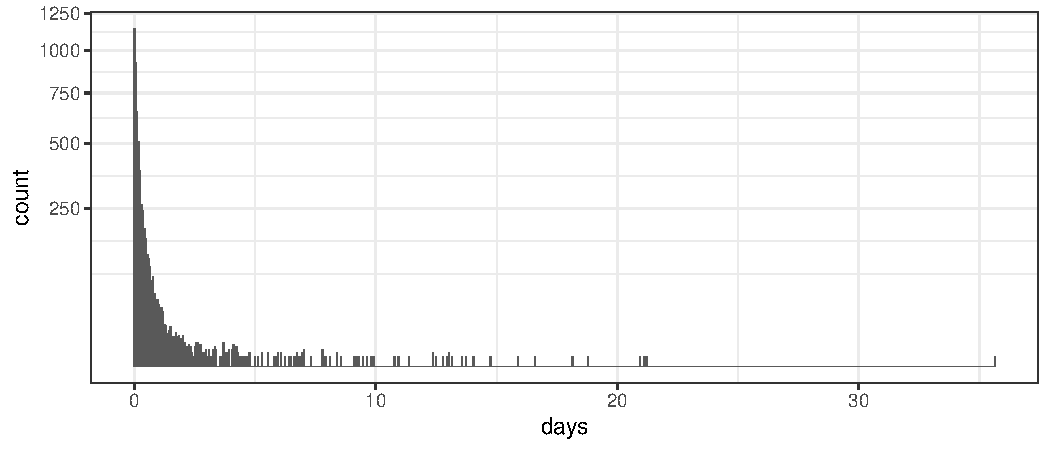
\includegraphics[width=\textwidth]{figs/attention_intervals001.pdf}
  \end{center}
  \caption{Inter-inventory times, obrained by taking intervals between
    unique dates in the data. Note square root scale on $y$-axis.}
  \label{fig:inventory}
\end{figure}
\fix{George: Add color for another variable? (new-old, date)??}
Notably, there was a period of over a month that Titan operated
without a single reboot.

Initial processing updates an inventory by checking the Serial Number
(SN) and Location of each GPU and creating or updating a separate
record for each contiguously observed SN-Location combination.


A typical GPU data record is of the form shown in Fig.~\ref{fig:dataraw},
\begin{figure}
{\small
\begin{verbatim}
0323812007945 | c17-4c1s3n1 | 01/10/2013 02:54:45 | 02/02/2013 11:32:29
 | c13-1c1s3n3 | 01/21/2014 21:10:42 | 08/01/2017 02:15:02
 | c0-1c1s3n3 | 10/11/2013 15:57:33 | 10/12/2013 22:09:31
 | c21-1c2s5n0 | 03/19/2013 15:48:11 | 05/29/2013 11:54:11
0325216047736 | c18-4c1s5n1 | 03/07/2017 02:15:01 | 03/12/2019 03:19:11
0323812008856 | c5-4c0s7n0 | 01/10/2013 02:54:45 | 01/25/2013 15:29:58
 | c0-6c1s7n2 | 10/21/2013 14:28:19 | 10/28/2013 17:52:44
 | c3-3c1s5n0 | 05/29/2013 11:54:11 | 05/29/2013 11:54:11
 | c23-6c1s7n2 | 01/21/2014 21:10:42 | 11/02/2018 14:42:34
 | | DBE | 11/02/2018 14:42:34
\end{verbatim}
}
\caption{A few records of raw data produced from inventories that is
  processed further in our analysis.}
\label{fig:dataraw}
\end{figure}
\noindent where records for three GPUs are shown. Each record starts
with a serial number and locations are coded with {\tt c{\it
    col-row}c{\it cage}s{\it slot}n{\it node}}. The first GPU record
shows installation in locations {\tt c17-4c1s3n1}, {\tt c21-1c2s5n0},
{\tt c0-1c1s3n3}, with periods off the system, and finally in {\tt
  c13-1c1s3n3}, where it stays until August 1, 2017, after which it is
not seen again. The second is intalled in location {\tt c18-4c1s5n1},
where it stays until the last data collection date on March 3, 2019,
at 3:19:11 AM. The third GPU is first installed in locations {\tt
  c5-4c0s7n0}, {\tt c3-3c1s5n0},{\tt c0-6c1s7n2}, {\tt c23-6c1s7n2},
where a ``DBE'' is observed on November 2, 2018, and it is not seen
again.
